%?????????????????????????
% Nombre: capitulo4.tex  
% 
% Texto del capitulo 4
%---------------------------------------------------

\chapter{T�cnicas fallidas}

En esta secci�n se hace un estudio de dos t�cnicas m�s de miner�a de datos cuyos resultados concluyeron que de cara al problema que nos incumbe no aportaban informaci�n suficiente (al menos al nivel estudiado) y por tanto fueron abandonadas y retiradas del grueso del trabajo general. 

\section{Reglas de asociaci�n}

Con el fin de poder mejorar los resultados obtenidos en \ref{forest}, se llev� a cabo un experimento de aplicaci�n de reglas de asociaci�n sobre el conjunto de entrenamiento para ver si podemos obtener algunas reglas interesantes cuyo consecuente sea \textit{\textbf{Vive}} o \textit{\textbf{Muere}}, y con las cuales podamos afinar nuestro proceso de aprendizaje. 

Para aplicar esto, de nuevo usamos Knime y el flujo que podemos ver en la figura \ref{fig_reglas}. Podemos notar, como hay un metanodo, denominado \textit{ReplaceNode} que aglutina cuatro nodos de \textit{RuleEngine} que realizan transformaciones en los datos para no tener que usar diccionarios externos y poder obtener reglas de asociaci�n entendibles f�cilmente. Estas reglas podemos verlas en las figuras \ref{r1}, \ref{r2}, \ref{r3} y \ref{r4}. 

\begin{figure}
	\centering
		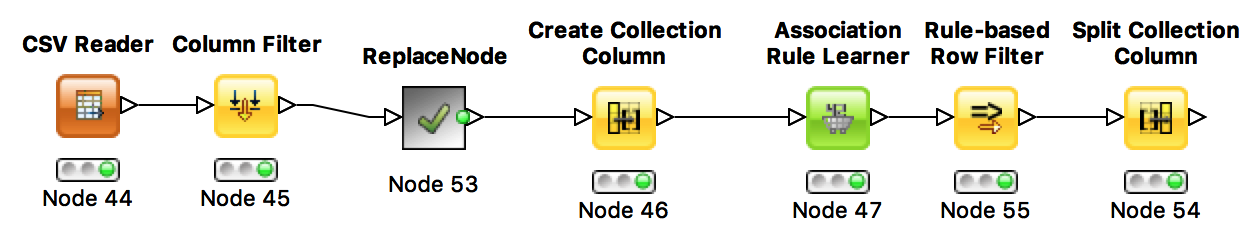
\includegraphics[scale=0.6]{./Capitulo4/imagenes/ar.png}
		\caption{Flujo de Knime para reglas de asociaci�n.}
	\label{fig_reglas}
\end{figure}

\begin{figure}
	\centering
		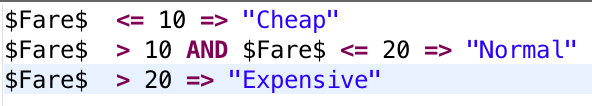
\includegraphics[scale=0.7]{./Capitulo4/imagenes/r1.png}
		\caption{Regla para categorizar Fare.}
	\label{r1}
\end{figure}

\begin{figure}
	\centering
		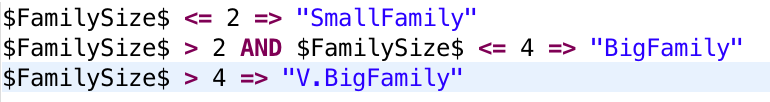
\includegraphics[scale=0.7]{./Capitulo4/imagenes/r2.png}
		\caption{Regla para categorizar FamilySize.}
	\label{r2}
\end{figure}

\begin{figure}
	\centering
		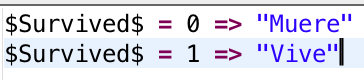
\includegraphics[scale=0.7]{./Capitulo4/imagenes/r3.png}
		\caption{Regla para categorizar Survived.}
	\label{r3}
\end{figure}

\begin{figure}
	\centering
		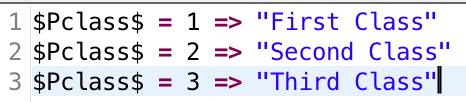
\includegraphics[scale=0.7]{./Capitulo4/imagenes/r4.png}
		\caption{Regla para categorizar Pclass.}
	\label{r4}
\end{figure}


Tambi�n se hace uso de un nodo RuleBasedFilter para quedarnos solo con las reglas que tienen en el consecuente \textit{\textbf{Vive}} o \textit{\textbf{Muere}} y de esta manera poder estudiar mejor el problema que nos incumbe. Tras la ejecuci�n del anterior flujo, obtenemos multitud de reglas de asociaci�n, pero todas las que tienen niveles de confianza aceptables tienen que ver con \textit{\textbf{vive si se es mujer}}. Algo que ya sab�amos a priori, por lo que a un nivel de confianza y soporte confiable, las reglas de asociaci�n no nos aportan nada que no hubi�ramos aportado ya al problema en anteriores pasos por lo que este m�todo ser� descartado. 

\begin{figure}
	\centering
		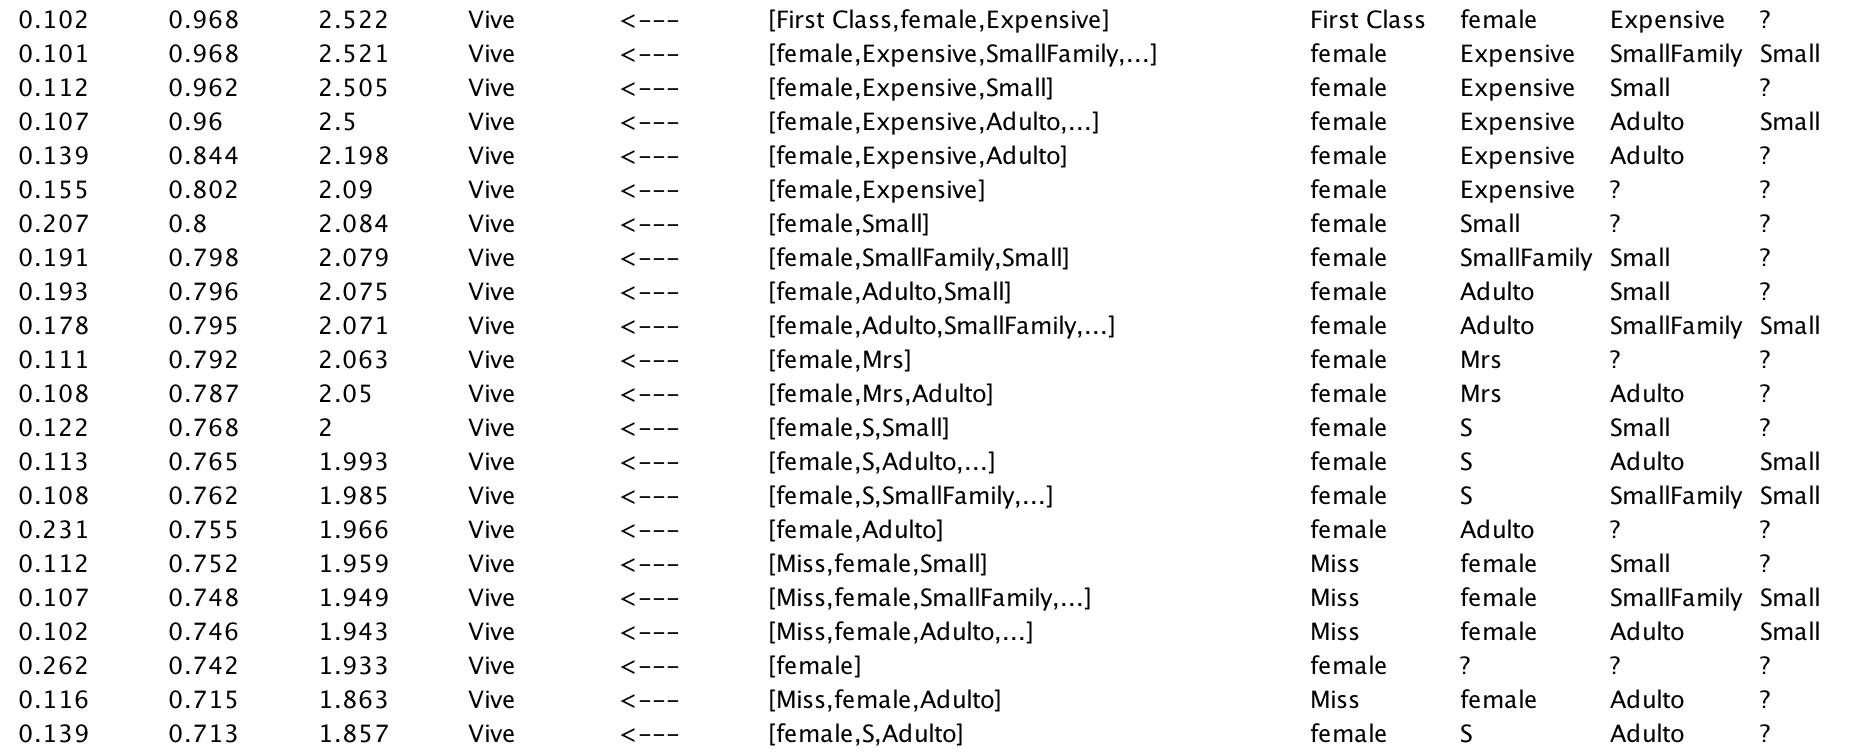
\includegraphics[scale=0.4]{./Capitulo4/imagenes/reglas.png}
		\caption{Reglas obtenidas.}
	\label{reglas}
\end{figure}


\section{Oversampling}

Si atendemos a la imagen , podemos ver que la distribuci�n de clases en el problema estudiado est� bastante desequilibrada teniendo casi el doble de muestras de la clase \textit{survived=0} frente a la clase \textit{survived=1}. Esto puede hacer que nuestros clasificadores ofrezcan cierto sesgo hacia la clase mayoritaria, frente a la minoritaria y en nuestro caso donde como hemos podido comprobar, el error en la clase \textit{survived=0}  es menor que en la \textit{survived=1} , ser�a menester eliminar este sesgo y comenzar a clasificar bien muestras de supervivientes para mejorar los resultados alcanzados tras nuestro proceso de clasificaci�n. 

Para favorecer esto, una t�cnica com�nmente usada es la denominada como \textit{oversampling} \cite{over} que crea muestras ficticias de la clase minoritaria para igualarlas frente a la mayoritaria y as� eliminar el sesgo anteriormente mencionado. Knime incluye una de estas t�cnicas, concretamente la que hace uso del algoritmo \textbf{SMOTE}.

Por tanto, haremos uso del flujo en Knime que vemos en la figura \ref{fig_smote} para a�adir nuevas muestras al conjunto de entrenamiento inicial, tras lo cual pasaremos de nuevo a R, para aplicarle las t�cnicas que describimos en el punto \ref{1}.


\begin{figure}[h]
	\centering
		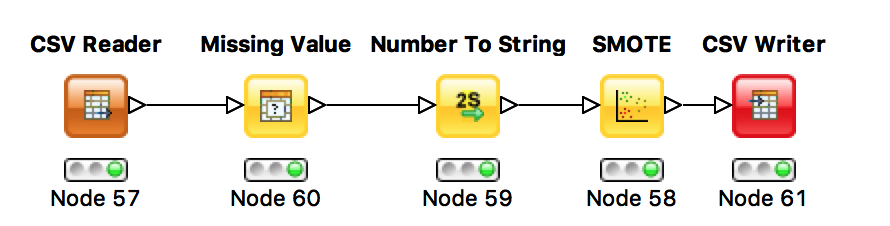
\includegraphics[scale=0.7]{./Capitulo4/imagenes/1.png}
		\caption{Flujo en Knime para aplicar oversampling.}
	\label{fig_smote}
\end{figure} 

Una vez aplicado de nuevo el algoritmo RandomForest visto en \ref{forest} y subir los datos a Kaggle para su evaluaci�n con el conjunto de test podemos comprobar que el resultado no es el esperado sino que se empeora respecto a lo entregado anteriormente. Tras un an�lisis de lo que ha ocurrido y porque no mejoramos el accuracy del sistema, podemos concluir en la siguiente explicaci�n:

El algoritmo \textbf{SMOTE}, crea muestras ficticias en funci�n de los datos de los que disponemos y les asigna la clase minoritaria hasta igualarlos. Notemos como tenemos un listado de pasajeros de los cuales la mayor�a no sobreviven al accidente, y en base a datos cuyo valor es survived=0, se crean nuevas muestras con esos datos (que como hemos dicho corresponden a survived=0 en su mayor�a) y se les asigna la clase survived=1, previa combinaci�n de atributos. En este problema concreto donde tenemos una gran influencia del factor aleatorio, este m�todo no hace por tanto otra cosa que confundir al algoritmo clasificador, por lo que esta t�cnica se desech�. 

\pagebreak
\clearpage
%---------------------------------------------------